\section{实际应用案例}

\subsection{社交网络分析}
图数据库在社交网络分析中被广泛应用,其核心特性是能够直观地存储和高效地查询节点之间的复杂关系。在社交网络中,用户被表示为节点,用户之间的社交关系(如好友关系、关注关系)被表示为边,这使得图数据库能够自然地建模并高效管理这些数据。

\begin{figure}
    \centering
    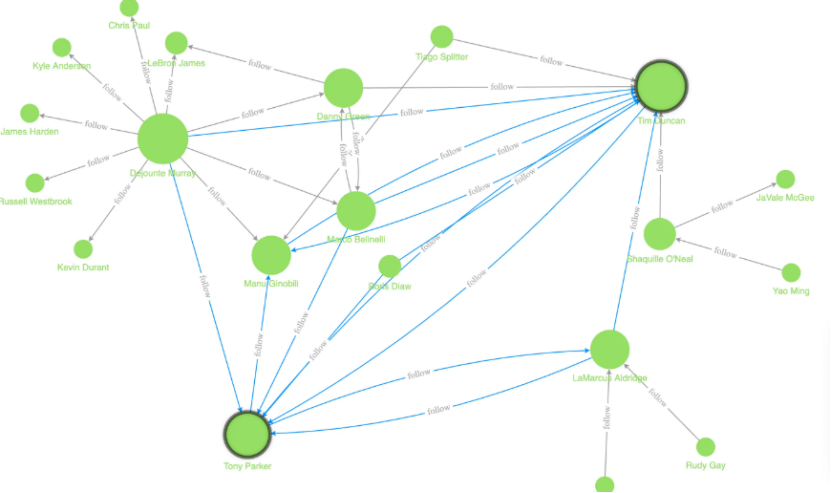
\includegraphics[width=0.8\textwidth]{images/24.png}
    \caption{社交网络分析}
    \label{fig:24}
\end{figure}
\textbf{好友推荐}:图数据库如 Neo4j 能够通过遍历社交图,实时地向用户推荐新的朋友。利用 Cypher 查询语言,Neo4j 可以在极短的时间内找到用户的好友的好友,计算可能认识的人,从而实现好友推荐功能。例如,在 Facebook 的社交网络中,实时推荐基于节点之间的距离和共同好友数\cite{ahmad2020missing,wang2022common}。


\textbf{社区检测}:图数据库还被用于检测社交网络中的社区(Community Detection),例如使用 Louvain 算法来发现社交群体。TigerGraph 提供了内置的社区发现算法,可以快速地找到由相互关联的节点组成的社交团体,这对社交广告投放和用户兴趣挖掘非常有帮助\cite{tsitseklis2020scalable,beis2015benchmarking}


\subsection{欺诈检测}
图数据库在金融和电子商务的欺诈检测中发挥着重要作用,尤其是在复杂关系的识别和实时查询方面。如\cref{fig:21}所示,欺诈行为通常伴随有多个实体之间的复杂交易记录和网络关系,图数据库可以快速识别其中的潜在欺诈模式
\begin{figure}
	\centering
	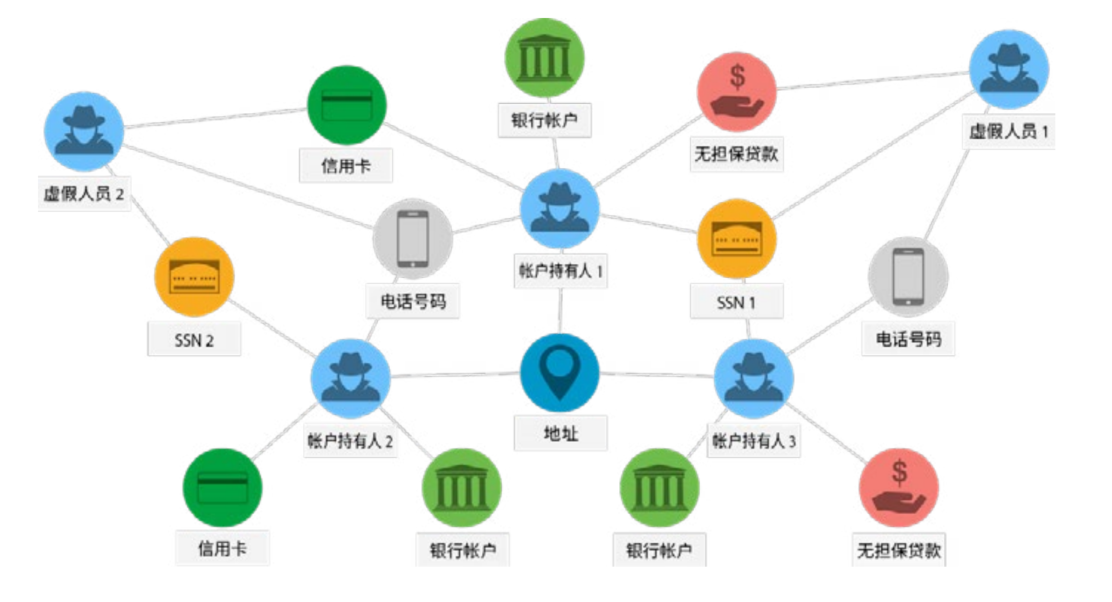
\includegraphics[width=0.8\textwidth]{images/21.png}
	\caption{欺诈检测}
	\label{fig:21}
\end{figure}

\textbf{多跳关系追踪}:在欺诈检测中,图数据库能够利用其高效的多跳查询能力,追踪交易链中可能的欺诈行为。例如,TigerGraph 在欺诈检测中能够通过图遍历快速发现潜在的欺诈路径,从而有效识别复杂的欺诈环节和背后的共谋关系。这种能力在银行交易和电子支付领域尤为重要,因为欺诈行为往往涉及多层代理账户和跨越多次交易\cite{mao2022financial,cheng2020graph,li2022internet}。

\textbf{实时风险评估}:图数据库中的实时查询功能可以用于实时的风险评估,例如,当一笔交易发生时,Neo4j 可以立即查询该账户的交易历史及其关联账户,从而实时判断是否存在风险。这种实时欺诈检测的能力对金融机构而言非常重要,可以有效防止欺诈交易的发生


\subsection{知识图谱}
知识图谱是一种用来表示实体及其关系的语义网络,图数据库在构建和管理知识图谱中扮演着不可或缺的角色。知识图谱通常用于知识管理、搜索引擎和问答系统中\cite{黄恒琪2019知识图谱研究综述}。
\begin{figure}
    \centering
    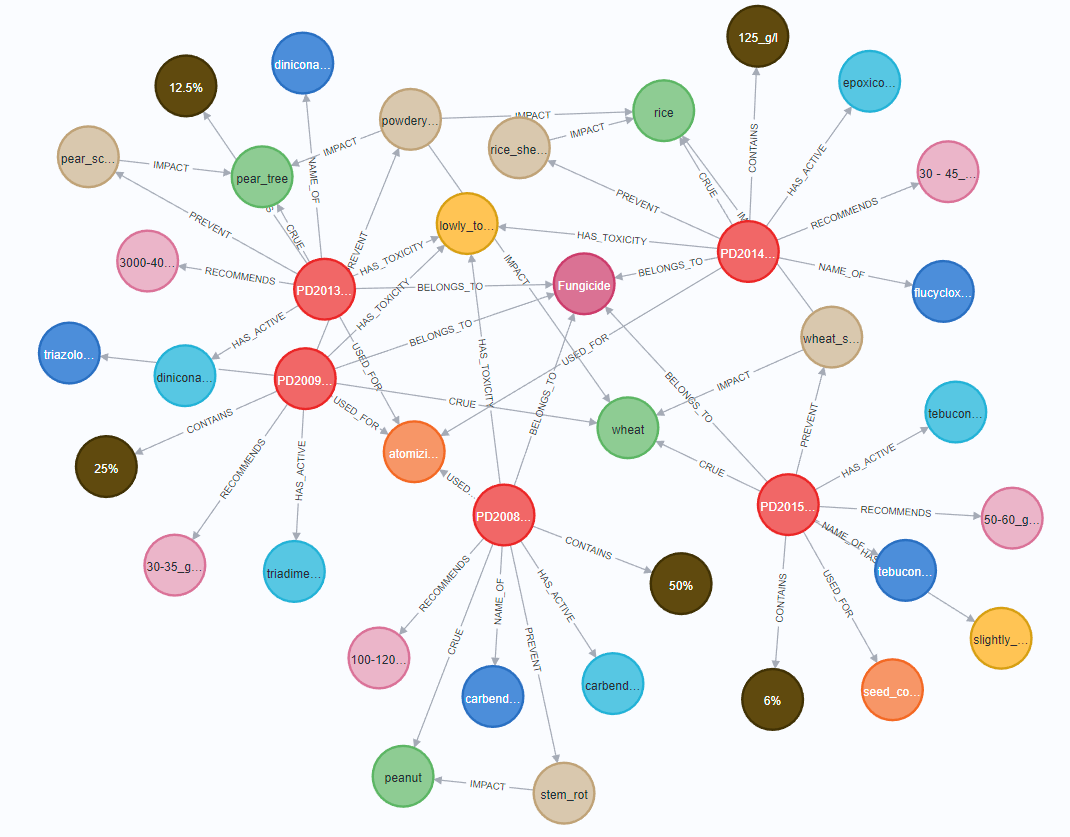
\includegraphics[width=0.8\textwidth]{images/23.png}
    \caption{农药知识图谱}
    \label{fig:23}
\end{figure}

\textbf{语义关系存储与查询}:图数据库的 RDF 模型非常适合知识图谱的存储和查询。例如,Google Knowledge Graph 使用图数据库来存储和管理不同实体之间的语义关系,以增强搜索引擎的智能化水平。通过使用类似 Cypher 或 SPARQL 的查询语言,知识图谱可以被高效查询以回答用户的问题\cite{dong2014knowledge}。

\textbf{实体链接与推理}:图数据库的特性允许知识图谱中进行实体链接和推理。TigerGraph 支持复杂的图分析算法,可以在知识图谱中进行推理,从而找到不同实体之间的潜在关系。这种推理被广泛应用于学术研究、医药领域以及产品推荐中,以更好地理解实体间的隐性关联\cite{徐增林2016知识图谱技术综述}。


\subsection{推荐系统}
推荐系统是图数据库的又一重要应用场景,尤其是在内容推荐、商品推荐等个性化推荐领域中表现出色\cite{秦川2020基于知识图谱的推荐系统研究综述,刘佳玮2021基于异质信息网络的推荐系统研究综述}。
\begin{figure}
    \centering
    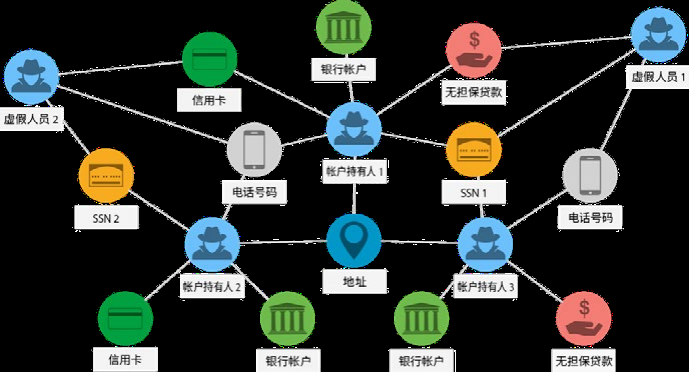
\includegraphics[width=0.8\textwidth]{images/22.png}
    \caption{推荐系统}
    \label{fig:22}
\end{figure}

\textbf{基于路径的推荐}:在电商平台中,图数据库可以通过计算用户与商品之间的关系路径,找出与用户兴趣最相关的商品,从而进行推荐。例如,eBay 使用图数据库来实现商品的个性化推荐,通过遍历用户的购买历史和兴趣图谱,找到与之相关的商品进行推荐。这种基于路径的推荐系统利用了图数据库高效的图遍历能力,可以在大量商品和用户关系中找到最优的推荐结果\cite{fayyaz2020recommendation,wu2022graph,赵俊逸2021协同过滤推荐系统综述}。

\textbf{社交推荐}:通过分析用户与用户之间的关系,图数据库可以实现社交推荐。Neo4j 的社交推荐功能能够利用用户之间的社交关系,例如“朋友购买了某商品”来推荐商品。这种推荐机制不仅能提高推荐的相关性,还能够基于社交信任来提升用户接受推荐的可能性\cite{fayyaz2020recommendation,赵俊逸2021协同过滤推荐系统综述}。


